\documentclass[12pt]{article}
\usepackage{tikz}
\usepackage[utf8]{inputenc}
\usepackage{listings}
\usepackage{ amssymb }
\usepackage{color}
\usetikzlibrary{automata,positioning,arrows}

\title{Estructura de datos y teoría de algoritmos\\
Tarea 2 }
\author{Fabián Romero}

\begin{document}
\lstset{language=python}
\maketitle

\section{Teorema de Landau}
\begin{itemize}
  \item[\bf{a)}] En el artículo de Griggs y Reid an Australasian Journal of Combinatorics 20 (1999), pp
19-24. Se describe la condición para que una secuencia sea de puntajes sea un torneo, en términos de coeficientes binomiales. Demuestra en detalle que si una secuencia es de
puntajes de un torneo, entonces satisface la condición.

  \item[Demostración:]
    Una secuencia de enteros $s=(s_1 \le s_2 \le .. \le s_n)$ es una secuencia de puntajes si:

 $\sum\limits_{i=1}^{k} s_i \ge {k \choose 2}, 1 \le k \le n $ y la igualdad se alcanza si $k = n$


    Demostración:

    Si una secuencia de puntajes es un torneo $T$, observe la gráfica $G$ de $n$ vértices que es el resultado de eliminar la dirección de cada arista, por ser un torneo tiene $n \choose 2$ aristas, pues cada 2 vértices estan conectados, luego, por constucción de la secuencia, cada arista es contada en el vértice de salida de la misma, así  $\sum\limits_{i=1}^{n} s_i = {n \choose 2}$ 

    para el caso $k < n$ basta notar que la gráfica inducida $T_k$ por los vértices $(v_1,v_2,..,v_k)$ corresponientes a la secuencia de puntajes, es también un torneo por lo que en $T_K$ se cumple que $\sum\limits_{i=i}^{k} s_i = {k \choose 2}$, por lo que en $T$ $\sum\limits_{i=i}^{k} s_i \ge {k \choose 2}$, pues todas las aristas de $T_k$ se conservan y podría haber vértices en la ex-vecindad de $T_k$ que contribuirán a la desigualdad $\blacksquare$

  \item[\bf{b)}]Presenta dos secuencias de 7 términos, una que satisfaga la condición del ejercicio anterior y otra que no. Se debe cumplir lo siguiente:
\begin{enumerate}
\item Ambas secuencias deben estar lo mas ``lejos'' posible de la secuencia transitiva.
\item La secuencia que no satisface la condición, debe parecer lo más posible que si la satisface.
\end{enumerate}

  \item[\bf{1}]
    considere la secuencia $(3,3,3,3,3,3,3)$

  \item[\bf{2}]
    considere la secuencia $(0,1,2,3,4,4,7)$

  \item[\bf{c)}] Describe como el algoritmo del artículo va tranformando la secuencia transitiva a tus dos secuencias propuestas en el inciso anterior, explicando claramente cada paso. Explica cómo detecta que la 2nda no es correcta.

  \item[\bf{Respuesta secuencia 1}]
    $(3,3,3,3,3,3,3)$
    se toman los elementos $0$ y $1$ que son iguales, se decrementa el primero y se incrementa el segundo\\
    $(2,3,3,3,3,3,4)$
    se toman los elementos $1$ y $2$ que son iguales, se decrementa el primero y se incrementa el segundo\\
    $(2,2,3,3,3,4,4)$
    se toman los elementos $0$ y $1$ que son iguales, se decrementa el primero y se incrementa el segundo\\
    $(1,3,3,3,3,4,4)$
    se toman los elementos $2$ y $3$ que son iguales, se decrementa el primero y se incrementa el segundo\\
    $(1,2,3,3,4,4,4)$
    se toman los elementos $2$ y $3$ que son iguales, se decrementa el primero y se incrementa el segundo\\
    $(1,2,2,4,4,4,4)$
    se toman los elementos $1$ y $2$ que son iguales, se decrementa el primero y se incrementa el segundo\\
    $(1,1,3,4,4,4,4)$
    se toman los elementos $0$ y $1$ que son iguales, se decrementa el primero y se incrementa el segundo\\
    $(0,2,3,4,4,4,4)$
    se toman los elementos $3$ y $4$ que son iguales, se decrementa el primero y se incrementa el segundo\\
    $(0,2,3,3,4,4,5)$
    se toman los elementos $2$ y $3$ que son iguales, se decrementa el primero y se incrementa el segundo\\
    $(0,2,2,4,4,4,5)$
    se toman los elementos $1$ y $2$ que son iguales, se decrementa el primero y se incrementa el segundo\\
    $(0,1,3,4,4,4,5)$
    se toman los elementos $3$ y $4$ que son iguales, se decrementa el primero y se incrementa el segundo\\
    $(0,1,3,3,4,5,5)$
    se toman los elementos $2$ y $3$ que son iguales, se decrementa el primero y se incrementa el segundo\\
    $(0,1,2,4,4,5,5)$
    se toman los elementos $3$ y $4$ que son iguales, se decrementa el primero y se incrementa el segundo\\
    $(0,1,2,3,5,5,5)$
    se toman los elementos $4$ y $5$ que son iguales, se decrementa el primero y se incrementa el segundo\\
    $(0,1,2,3,4,5,6)$
    y finalmente, despues de 14 pasos, queda la secuencia transitiva 

  \item[\bf{Respuesta secuencia 2}]

    $(0,1,2,3,4,4,7)$
    se toman los elementos $4$ y $5$ que son iguales, se decrementa el primero y se incrementa el segundo\\
    $(0,1,2,3,3,5,7)$
    se toman los elementos $3$ y $4$ que son iguales, se decrementa el primero y se incrementa el segundo\\
    $(0,1,2,2,4,5,7)$
    se toman los elementos $3$ y $4$ que son iguales, se decrementa el primero y se incrementa el segundo\\
    $(0,1,1,3,4,5,7)$
    se toman los elementos $3$ y $4$ que son iguales, se decrementa el primero y se incrementa el segundo\\
    $(0,0,2,3,4,5,7)$

    Y ahi encuentra que los primeros 2 elementos son 0, el paso siguiente seria cambia el primero por -1 y el segundo por 1, pero eso no hace sentido, y así detecta que no es correcta.

  \item[\bf{d)}]
Haciendo pruebas y usando cada vez el arreglo con mas elementos iguales toma:

$0, 0, 1, 2, 5, 8, 14, 20, 30, 40, 55, 70, 91, 112, 140, 168, 204, 240...$ pasos con n elementos, resolviendo la ecuación en diferencias nos da:

$a_n = {\frac{n}{48}}(2 n^2-3 (-1)^n-5)$ lo cual es $\theta(n^3)$
 


\end{itemize}
\section{Dijkstra.}
\begin{itemize}

  \item[\bf{a)}]
ee el capitulo de Dijkstra del libro Out of Their Minds de Shaha y Lazere y presenta
un resumen de una o dos cuartillas que explique en que problemas trabajo, como era
su personalidad, y como explicarias que tiene de especial o que lo distingue de otros
grandes científicos de la computación

  \item[\bf{Respuesta}]

En cuanto a su personalidad, el mismo se describe como una persona extremadamente consistente. Es evidente a partir del texto la asombrosa claridad de su mente, nos presenta 3 trabajos importantes, uno es aquel del algoritmo que se conoce por su apellido que nos permite encontrar la ruta óptima en una gráfica con pesos en las aristas,  Edgar Dijkstra se adelanto a su tiempo y lo resolvió cuando todavia estos temas no tenian mucha difusión, de hecho, no fue fácil encontrar quien lo publicara y sin embargo, hoy en día es de gran relevancia y central en el área de algoritmos, sería muy difícil hoy en dia encontrar un libro en este tema que no lo incluyera, también anecdóticamente cuentan como lo resolvió en una sola sentada y en la cabeza, no es sin embargo menos notable la elegancia, pues si resolver el problema es por si meritorio, encontrarlo es mayormente importante, especialmente uno que sea tan representativo.

El segundo trabajo que nos relata el texto, es el que se conoce como el ``problema de selección crítica'', que es referente al tema de cooperación y exclusión mutua en las operaciones sequenciales, el punto realmente relevante en este tema, es notar como, en su notable capacidad para abstraer, lo más importante es saber seleccionar los elementos que son realmente relevantes y desechar los que no, buscando la minimalidad de factores a considerar, en este caso, al considerar irrelevante el tiempo y relevante el rol de ``esperar'' mostro de nuevo, como una mente clara simplifica el problema hasta volverlo trivial y evidente una vez que se observa con la perspectiva adecuada.

El tercer y último trabajo que se presenta es  ``la cena de los filósofos'' donde plantea las situaciones de ``bloqueo'' y ``cooperación'' en elementos que dentro de un sistema adquieren recursos y como estos podrán cooperar. Aqui también resalta la mente clara que es capaz de comprender el verdadero problema subyaciente a la utilización concurrente de recursos  y capaz de esclarecer aquello que para el mundo resultaba obscuro y proponer como hacer programas demostrablemente correctos.

Aqui la mente clara de Dijkstra nos muestra la busqueda de la verdad y la belleza por medio de la simplicidad y la elegancia, la limpieza de los argumentos y la contundencia de la matemática como su herramienta.

  \item[\bf{b)}]
Demuestra que el algoritmo de Dijkstra no funciona en gráficas dirigidas que puedan
tener pesos negativos en los arcos. Presenta un ejemplo genérico en el que falla (es decir,
una gráfica de n vértices en general).

  \item[\bf{Respuesta}]
La redacción no es correcta, sería correcto decir: el algoritmo de Dijkstra no \emph{siempre} funciona en gráficas dirigidas que puedan tener pesos negativos en los arcos.
pues por ejemplo en una gráfica como la siguiente funciona bien el algoritmo:


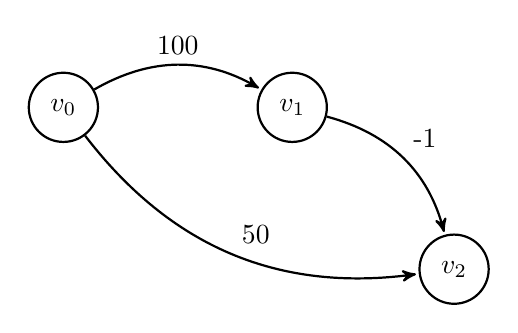
\begin{tikzpicture}[->,>=stealth',shorten >=1pt,auto,node distance=2cm,
  thick,main node/.style={circle,fill=blue!20,draw,font=\sffamily\Large\bfseries}]
   \node[state] (v_0)   {$v_0$}; 
   \node[state] (v_1)  [right=of v_0] {$v_1$}; 
   \node[state] (v_2)  [below right=of v_1] {$v_2$};
    \path[->] 
    (v_0) edge  [bend left]  node {100} (v_1)
          edge  [bend right] node {50} (v_2)
    (v_1) edge  [bend left] node  {-1} (v_2);
\end{tikzpicture}

Sin embargo el siguiente ejemplo falla con el algoritmo

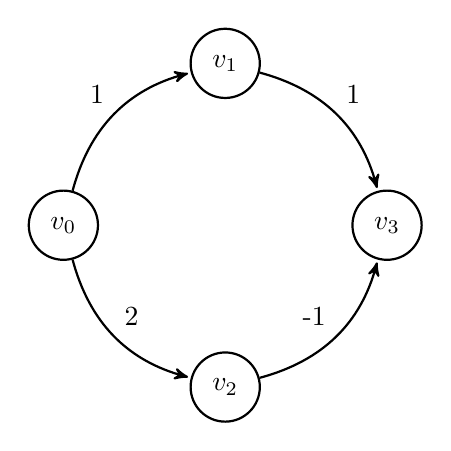
\begin{tikzpicture}[->,>=stealth',shorten >=1pt,auto,node distance=2cm,
  thick,main node/.style={circle,fill=blue!20,draw,font=\sffamily\Large\bfseries}]
   \node[state] (v_0)   {$v_0$}; 
   \node[state] (v_1)  [above right=of v_0] {$v_1$}; 
   \node[state] (v_2)  [below right=of v_0] {$v_2$};
   \node[state] (v_3)  [below right=of v_1] {$v_3$};
    \path[->] 
    (v_0) edge  [bend left]  node {1} (v_1)
          edge  [bend right] node {2}  (v_2)
    (v_1) edge  [bend left] node  {1} (v_3)
    (v_2) edge  [bend right] node  {-1} (v_3);
\end{tikzpicture}

Pues partiendo de $v_0$, llega a $v_3$ por medio de $v_1$ que tiene un costo total $2$.
Sin embargo, si encontrara a $v_3$  por medio de $v_2$ tendría un costo total de $1$ que es mejor. Este ejemplo sirve bien para el caso de $n$ nodos, pues basta considerar dos caminos en este caso $(v_0,v_1,v_3)$ y $(v_0,v_2,v_3)$, pero bien podrían ser $(v_0,v_1,..v_k,..,v_n)$ y $(v_0,v_2,..,v_k,...v_n)$,  donde uno tenga una componente negativa al final que resulte en una suma menor que el primero, pero solo al final. 

\end{itemize}

\section{Ford.}
\begin{itemize}
  \item[\bf{a)}] Demuestra que el algoritmo de Ford funciona en una digráfica en la cual puede haber pesos negativos en los arcos, pero no hay ningún ciclo de peso negativo al cual se pueda llegar desde s. También que al terminar, calcula correctamente la distancia de s a todos
los demás vértices.

\item[\bf{b)}] Explica por qué el algoritmo es de complejidad exponencial.
  
\item[\bf{c)}] Demuestra que en la versión avanzada, la complejidad es orden de n por m, donde n es
el número de vértices y m el número de arcos.

\item[\bf{d)}] Explica como utilizar esta versión para detectar si hay un ciclo de peso negativo alcanzable desde s.

\end{itemize}
\end{document}
